\chapter{Описание  решения}

\label{cha:Solution}
 
\section{Разработка сценариев работы ``умного освещения''}
\subsection{Регистрация устройства}

Под регистрацией устройства мы будем понимать привязывание устройства к аккаунту пользователя. Для того, чтобы привязать устройства к аккаунту пользователя необходимо передать устройству пароль и название сети Wi-Fi. Для этого пользователь подключается к сетки, которую раздает устройство, через мобильное приложение и следует всем инструкциям

Пользователь выбирает опции добавить новое устройство и выполняет все необходимые шаги, для того чтобы в дальше использовать это устройство. Устройство должно установить, что владельцем устройства является именно этот пользователь. Сервер должен установить, что именно этот пользователь владеет именно этим устройством.

Действующие лица:	Устройство, Сервер, Пользователь, 
Приложение

Цель:	Связать устройство и аккаунт пользователя

Условие:	Пользователь авторизован в мобильном приложении, устройство включено и раздает свою сеть

Результат:	Мобильное приложение может управлять устройством

Успешный сценарий (рисунок \ref{fig:pic_useCase1})
\begin{itemize}
    \item Пользователь считывает код от устройства
    \item Пользователь выбирает опцию "добавить устройство"
    \item Пользователь вводит код от устройства в соответсвующее поле ввода
    \item Приложение ищет wi-fi сеть устройства в соответсвии с введенным кодом
    \item Приложение подключается в wi-fi сети устройства
    \item Пользователь вводит название домашней сети wi-fi, а также передает пароль от нее
    \item Приложение передает устройству название сети и пароль от нее
    \item Устройство подключается к домашней сети
    \item Устройство перестает раздавать свою сеть
    \item Устройство передает на сервер информацию о реализованной регистрации
    \item Приложение проверяет у сервера статус регистрации
    \item Сервер сохраняет информации о пользователе и об устройстве зарегистрированном за этим пользователем
\end{itemize} 


\begin{figure}[ht]
   \centering
   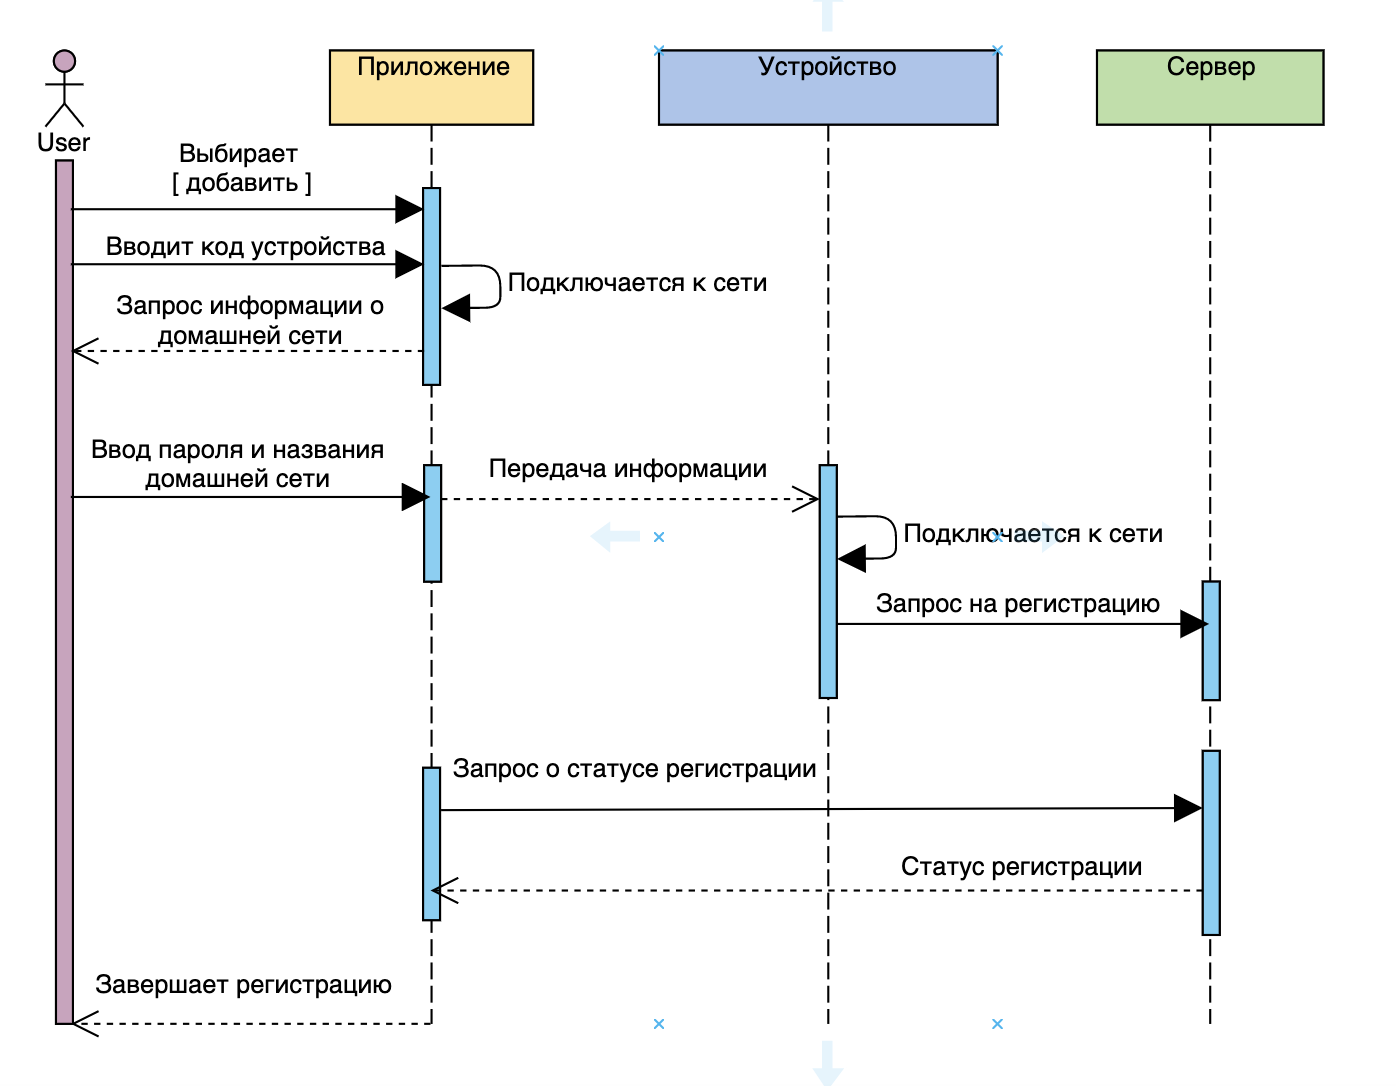
\includegraphics[scale=.5]{figures/pic_useCase1}
    \caption{UseCase 1}
    \label{fig:pic_useCase1}
\end{figure}

\subsection{Забыть устройство}
Пользователь может отвязать устройство от своего аккаунта. Например, если устройство больше не будет использоваться или в тех ситуациях, когда пользователь хочет привязать устройство к другому устройству.

Действующие лица	Устройство, Сервер, Пользователь, Приложение
Цель	Отвязать устройство от аккаунта пользователя
Условие	Пользователь ранее регистрировал устройство на свой аккаунт
Результат	Мобильное устройство забывает об устройстве, а устройство возвращается в изначальное состояние

Успешный сценарий (рисунок \ref{fig:pic_useCase2})
\begin{itemize}
    \item Пользователь выбирает удаление конкретного устройства
    \item Приложение отправляет устройству соответствующий запрос
    \item Приложение отправляет серверу соответсвующий запрос
    \item Приложение удаляет информацию об устройстве
    \item Приложение уведомляет пользователя об успешном завершении операции
\end{itemize}

\begin{figure}[ht]
   \centering
   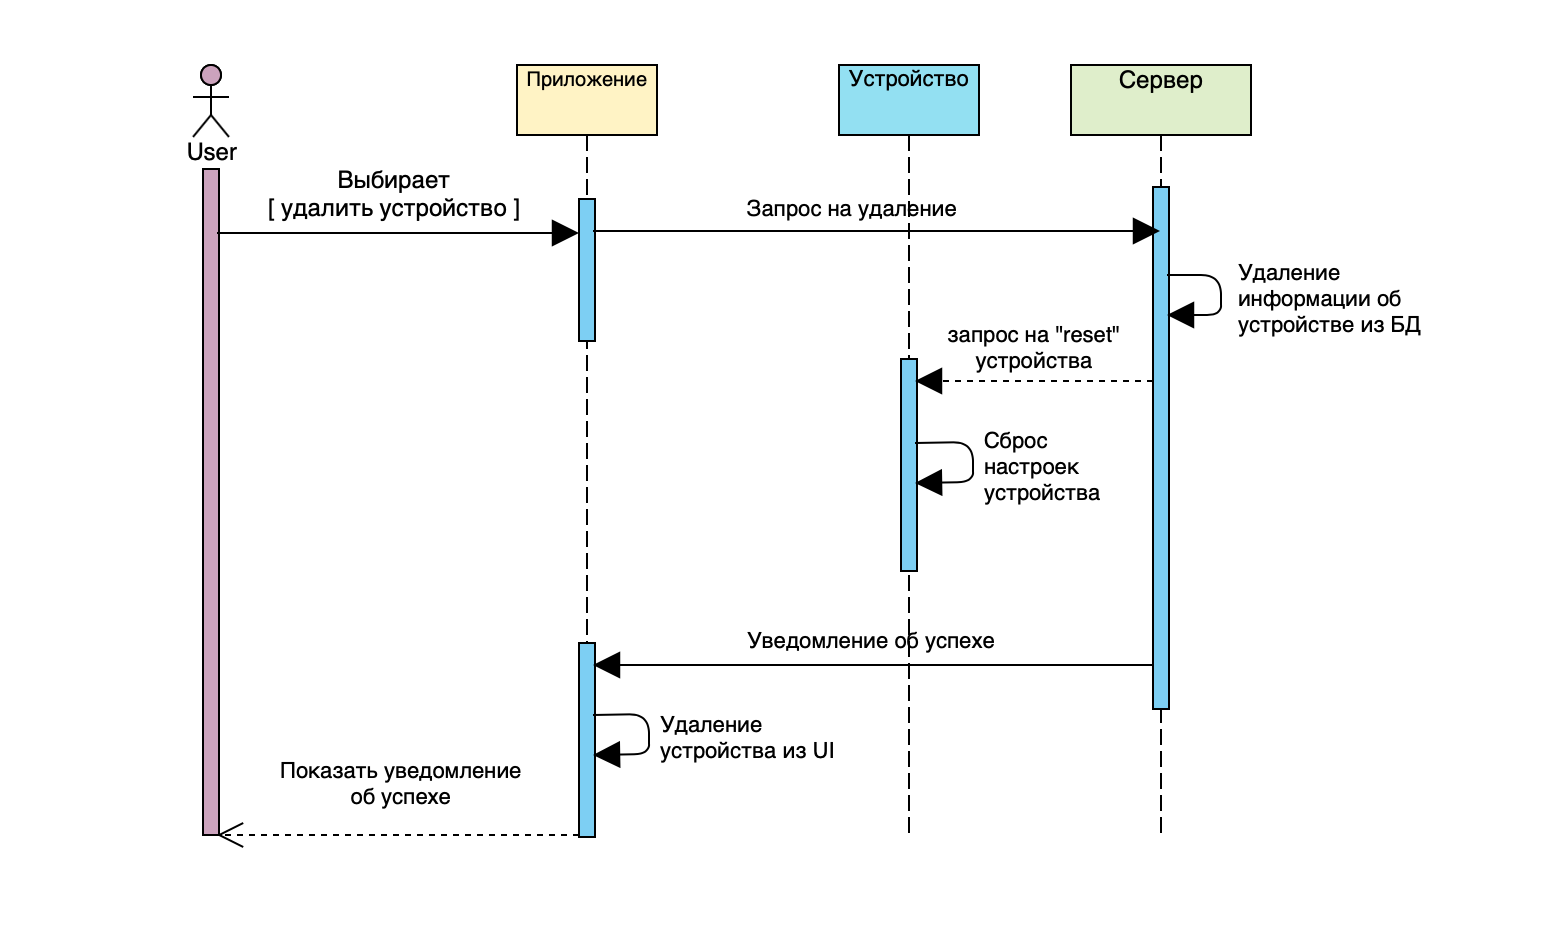
\includegraphics[scale=.5]{figures/pic_useCase2}
    \caption{UseCase 2}
    \label{fig:pic_useCase2}
\end{figure}

\subsection{Посмотреть список устройств управляемых с мобильного приложения}
Пользователь может посмотреть список устройств, которые он ранее зарегистрировал в мобильном приложении. Информация об устройствах хранится в базе данных мобильного устройства, которая обновляется из облака.

Описание сценария приведено на рисунке \ref{fig:pic_useCase3}.


    Для обновления информации о списке устройство на сервер делается HTTP запрос
    Приложение для каждого устройства должно отображать:
\begin{itemize}
    \item иконку, которая однозначно определяет тип устройства 
    \item название устройства
    \item уровень заряда (для устройств имеющих такой параметр)
    \item доступность устройства
    \item активное ли устройство.
\end{itemize}


\begin{figure}[ht]
   \centering
   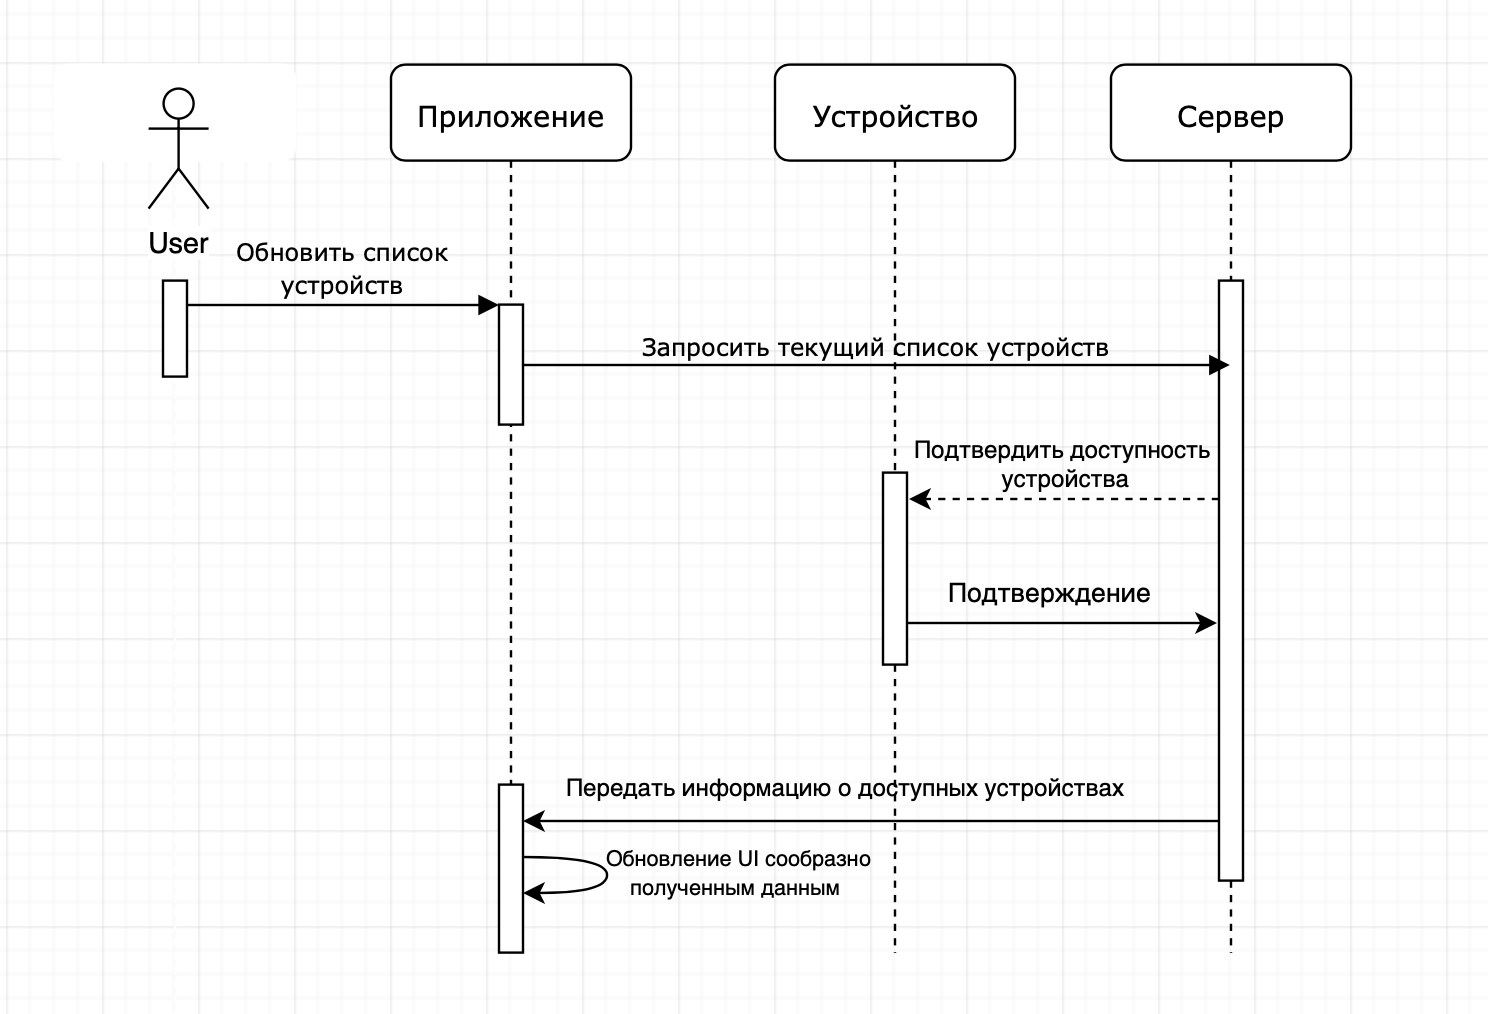
\includegraphics[scale=.5]{figures/pic_useCase3}
    \caption{UseCase 3}
    \label{fig:pic_useCase3}
\end{figure}

\subsection{Просмотр доступных сценариев}

Пользователь может просматривать доступные для установки на устройство сценария. Список сценариев хранится в базе данных устройства, которая обновляется из облака по запросу от мобильного приложения

Для обновления информации о списке доступных сценариев на сервер делается HTTP запрос

Приложение для каждого устройства должно отображать:
\begin{itemize}
 \item название сценария
  \item иконку сценария
\end{itemize}


\begin{figure}[ht]
   \centering
   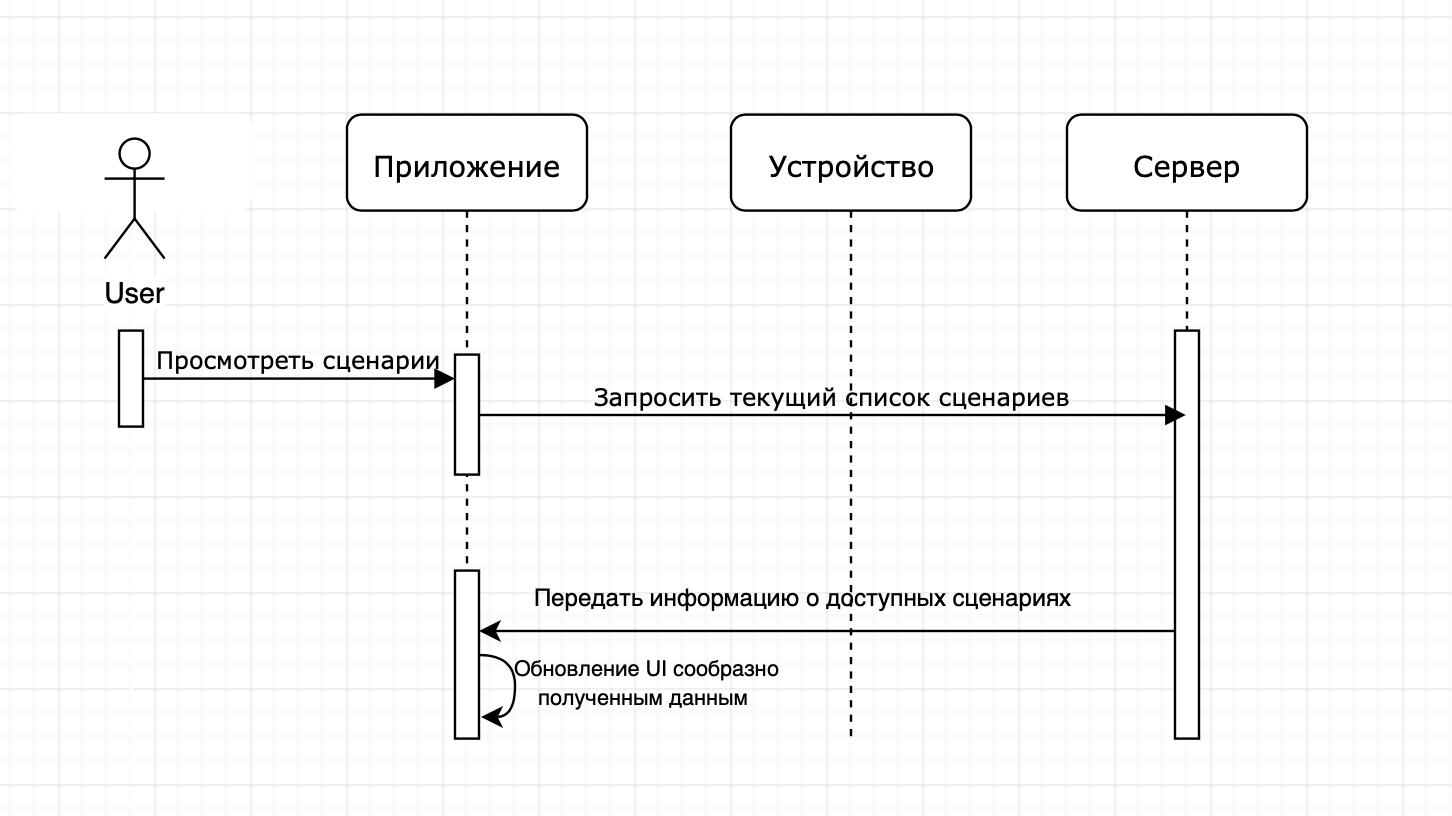
\includegraphics[scale=.5]{figures/pic_useCase4}
    \caption{UseCase 4}
    \label{fig:pic_useCase4}
\end{figure}

\subsection{Запуск сценария}  
Команда \verb|POST /device/<id>/scenario| - производит запуск сценария на устройстве с id=<id>. В качестве параметров передается JSON имеющий следующие поля:
\begin{itemize}
\item model - Тип String, модель осветительного устройства.
\item looped - Тип Bool, принимает значения:
true - если сценарий является зацикленным (то есть воспроизводящимся вновь по окончанию),
false - если сценарий не является зацикленным (то есть устройство не воспроизводит светомузыку по окончанию сценария)
\item method - Тип String, название метода, который нужно произвести с устройством. Может принимать два значения:
switch\_mod - На устройстве будет воспроизведен некоторый сценарий.
turn\_off - Устройство погаснет.
\item params - Тип Map, содержит описание сценария. См ниже Атрибуты сценария
\item brightness - Тип Float, яркость, принимает значения от 0 до 1.0
\item duration - Тип Int, длительность сценария в миллисекундах
\end{itemize}
Пример JSON:
\begin{verbatim}
request
{
 "model": "COSGarland_1",
 "looped": true,
 "method": "switch_mode",
 "params": [
  "mode": "double_color",
  "color1": "red",
  "color2": "white"
 ],
 "brightness": 0.5,
 "duration": 20,
}   
\end{verbatim}


\subsubsection{Атрибуты сценария}

Поле params содержит в себе основную информацию о сценарии, который будет воспроизведен. params содержит в себе:

mode - Тип String, название сценария. (Полный список сценариев см ниже Виды сценариев)

color1 - Тип String, Цвет 1, принимающий участие в светомузыке. Принимает значения: (red, green, white etc...)

color2 - Тип String, Цвет 2, принимающий участие в светомузыке. Принимает значения: (red, green, white etc...)

period - Тип Int, Некоторый период в миллисекундах. Играет разные роли в зависимости от параметра mode.

\subsubsection{Виды сценариев}

Ниже приведены некоторые из возможных режимов работы гирлянды:

solid\_color - Гирлянда горит одним цветом

double\_color - Гирлянда горит двумя цветами: четные лампочки горят цветом 1, а нечетные цветом 2

fading - Гирлянда затухает, а затем загорается с заданным периодом

blinking - Гирлянда мигает заданным цветом с заданным периодом

running\_light - Лампочки гирлянды загораются по очереди сменяя друг друга с заданным периодом

random - Гирлянда воспроизводит некую случайную последовательность световых сигналов


 
\section{Разработка API облачного сервера}
  
\section{Разработка формата описания сценариев работы ``умной гирлянды''}  

Нами разработан общий способ описания любого сценария RGB гирлянды. Он представляет из себя XML со следующими полями:

scenario - Внутри этого тэга находится вся информация о сценарии

mode\_name - Тип String, Имя описываемого сценария

one\_period\_duration - Тип Int, длительность между итерациями свечения гирлянды в миллисекундах (Через сколько времени лампочки должны сменить цвет)

number\_of\_periods - Тип Int, число описанных выше итераций

lamp - Объект содержащий в себе состояния цвета лампы. Содержит один атрибут - color, это цвет в формате RGB.

state - Описывает состояние всей гирлянды в данный момент времени. Имеет собственный ID соответсвующий порядковому номеру соответствующего момента времени.

\begin{verbatim}
<?xml version="1.0" encoding="UTF-8"?>
<?xml-stylesheet href="garland.xsl" type="text/xsl" ?>
<scenario>
    <mode_name>Double color running light mode</mode_name>
    <one_period_duration>300</one_period_duration> 
    <number_of_periods>11</number_of_periods> 
    <state id = '0'>
	    <lamp color = '#123d8c'/>
        <lamp color = '#000000'/>
        <lamp color = '#000000'/>
        <lamp color = '#7d69b5'/>
        <lamp color = '#000000'/>
	</state>
    <state id = '1'>
	    <lamp color = '#000000'/>
        <lamp color = '#123d8c'/>
        <lamp color = '#000000'/>
        <lamp color = '#000000'/>
        <lamp color = '#7d69b5'/>
	</state >
        ...
    <state id = '11'>
        <lamp color = '#000000'/>
        <lamp color = '#000000'/>
        <lamp color = '#7d69b5'/>
        <lamp color = '#000000'/>
        <lamp color = '#000000'/>
	</state >
</scenario>
\end{verbatim}
